\section{Approach}
\label{section:approach}

%\begin{enumerate}
%	\item Präsentation eures Ansatzes
%	\item Meistens bietet es sich an erst die grobe Idee zu vermitteln und dann erst ins Detail zu gehen
%	\item Auf interessante und wichtige Design-Entscheidungen eingehen
%	\item Modelle einsetzen
%\end{enumerate}

In this section we first explain the setup we decided to use for fuzzing embedded devices. Furthermore, we explain the CoAP header fields more in-depth and how they are fuzzed.

\subsection{Setup}
Since we intended to fuzz a CoAP implementation running on a real IoT device, we needed to decide on a setup that enables us to properly send messages with a high throughput and to implement a fuzzer in an easy-to-use high-level language. Having these goals, we decided against fuzzing as an internal attacker from an embedded device in the IoT network, since it has limited resources compared to a desktop computer or laptop. It would also mean that we would need to implement the fuzzer in C, which would take us longer and it would be harder to implement features compared to a scripting language like Python.

We therefore decided to fuzz the IoT device as an external attacker from a laptop that is not part of the IoT network. To do so, we need to be able to communicate with the embedded device via IPv6, which is possible if we set up one OpenMote as a border router and a second one as a CoAP server. Via the border router, we can send messages with IPv6 into the IoT network and therefore send messages to the CoAP server. The CoAP server uses the Contiki-NG CoAP implementation and runs the Contiki-NG CoAP example server on the application layer. Since we only want to fuzz the CoAP implementation, it does not matter what the server on the application layer does with the payload of the CoAP messages. This setup is displayed in \Autoref{figure:fuzzing_setup}.

\begin{figure}[h]
	\centering		
	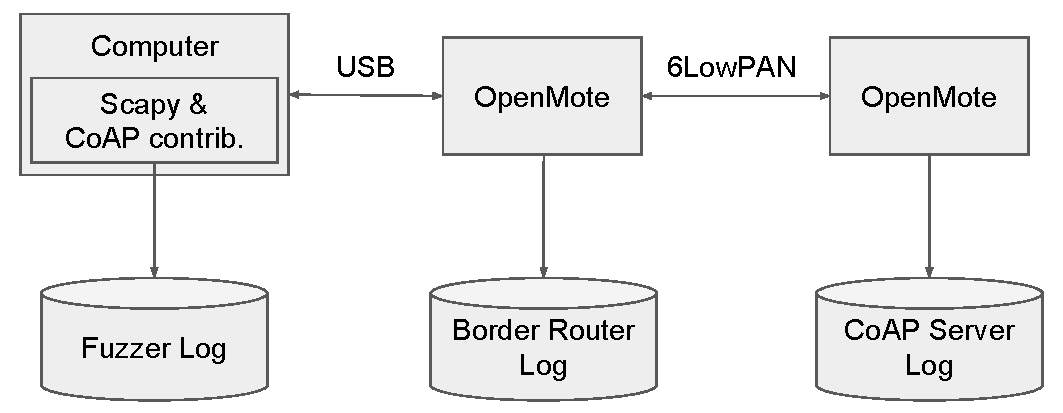
\includegraphics[width=0.5\textwidth]{images/fuzzing_setup}
	\caption{Setup of the embedded devices}
	\label{figure:fuzzing_setup}
\end{figure}

Having decided on the setup, we chose to implement the fuzzer in Python and similarly to Melo et al.~\cite{Melo2017RobustnessTO} we use \scapy to create crafted CoAP packets and send them to the IoT device. Our fuzzing workflow looks as follows. We first send a crafted packet to the CoAP server and await a possible response. After getting the response or getting a timeout (e.g., after sending a NON-message) we then test if the IoT device is still reachable or if it somehow does not respond to messages anymore (e.g., due to a crash or some other malfunction). 

\subsection{Fuzzing CoAP}
\begin{figure}[h]
	\centering		
	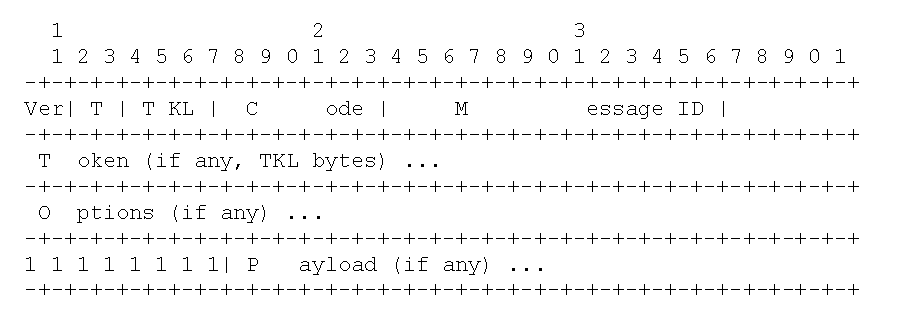
\includegraphics[width=0.5\textwidth]{images/coap_message_format}
	\caption{CoAP header fields defined in the CoAP RFC~\cite{RFC7252}}
	\label{figure:coap_header}
\end{figure}

After determining the message flow we now needed to decide how the craft the CoAP packets. We first read the CoAP RFC and analyzed the CoAP message header in \Autoref{figure:coap_header}. From the fuzzing approaches presented in \Autoref{section:background}, we chose generational fuzzing since we know the protocol being used. Contiki-NG is open source as well, which means that we can employ white-box fuzzing and verify how the header fields are handled and parsed. We further describe how we fuzz each header field:
\begin{enumerate}
	\item \textbf{Version}: there is currently only one version of CoAP so the version has to be always 1. Contiki-NG has a simple equality check for this field so there is no point in fuzzing this field.
	\item \textbf{Message Type}: since all four message types are valid we simply randomly fuzz this field.
	\item \textbf{Token Length}: this field contains the length of the token field, which is needed because CoAP has a lot of implicit field sizes in its header. The lengths 9 to 15 are reserved according to the RFC and Contiki-NG tests whether this field is larger than 8~\cite{RFC7252}. We therefore fuzz this field randomly in the range [0, 8].
	\item \textbf{Status Code}: every not implemented status code is simply caught by the implementation. Therefore, we randomly choose either a request or a response status code.
	\item \textbf{Message ID}: this id identifies CoAP messages for the purpose of deduplication and response matching. It has a random value anyway, which means that we do not gain anything by fuzzing this field. But we still need to set it randomly to be able to properly send and receive our crafted CoAP messages.
	\item \textbf{Token}: this field is practically the request id. The length of this field can differ from the token length field, since there are no well-defined boundaries for the following fields. That means it can not be checked if the token is too long or too short. We set this value randomly, but the byte length is independent from the value of the token length field.
	\item \textbf{Options}: CoAP options are parsed by reading the bytes after the token and trying to parse them as an option. These options each have small headers themselves, but unfortunately \scapy does enable us to fuzz these option headers as well.

	After an option was successfully parsed, the next byte is looked at and if it is not the payload marker, the following bytes are parsed as options as well. This goes on until a payload marker is found, which then means that after it, a payload with a non-zero lengths follows.

	We fuzz the CoAP options by randomly selecting a number of options implemented by Contiki-NG, which implements a few more options than those defined in the RFC~\cite{RFC7252}. The values for these options are random strings with a length of 0 to 12.
	\item \textbf{Payload}: the payload goes from the first byte after the payload marker to the last byte of the UDP datagram. Since the payload is not touched by the CoAP engine of Contiki-NG we do not fuzz it.
\end{enumerate}

The final decision we now have to make is how we want to detect if the IoT device crashed or malfunctioned after we sent it a crafted CoAP packet. We discussed the following approaches:
\begin{enumerate}
	\item \textbf{Pinging the device}: the simplest approach to test if a device is still reachable in a network is to ping it. This also works with our IoT devices but since an ICMP echo request is handled on the IP layer, it does not reach the CoAP layer and might be answered even though the CoAP engine somehow malfunctioned.
	\item \textbf{Well-known-core request}: according to the RFC, every CoAP server needs to implement the URI-route ``/.well-known/core``, which describes the resources provided by the server~\cite{RFC7252}. This basically acts as a CoAP ping for us, since it is a route every CoAP server has to provide and to respond to the request the CoAP engine is used. If the content of the response is known, the response after each fuzzing request can be tested for proper structure as well, i.e., that the returned content was not somehow changed by the CoAP engine malfunctioning.
	\item \textbf{Filter CLI output of CoAP server}: we can filter the standard output of the CoAP server for error messages and the log messages of the hardware watchdog, that restarts the device if it froze (e.g., in an infinite loop). We can then add timestamps to the whole standard output and match those with timestamps of the fuzzing requests.
	\item \textbf{Add logging to Contiki-NG}: since Contiki-NG is open source, it is possible to simply add more log output to the CoAP implementation to test, for example, memory content of the global buffers used by Contiki-NG.
	\item \textbf{JTAG debugging}: it is possible to attach a debugger via JTAG to the OpenMotes and read out all the memory. This also enables testing of the validity of the memory and to detect writing into sections of memory that should not be written to by the CoAP implementation.
\end{enumerate}

We decided to test the availability of the IoT device via the Well-known-core request, since it is the most straightforward way to check the reachability of the OpenMote and to check that the CoAP implementation still works.
